\documentclass{article} % For LaTeX2e
\usepackage{nips14submit_e,times}
\usepackage{amsmath}
\usepackage{amsthm}
\usepackage{amssymb}
\usepackage{mathtools}
\usepackage{hyperref}
\usepackage{url}
\usepackage{algorithm}
\usepackage[noend]{algpseudocode}
%\documentstyle[nips14submit_09,times,art10]{article} % For LaTeX 2.09

\usepackage{bbm}
\usepackage{graphicx}
\usepackage{caption}
\usepackage{subcaption}
\usepackage{MnSymbol}

\def\eQb#1\eQe{\begin{eqnarray*}#1\end{eqnarray*}}
\def\eQnb#1\eQne{\begin{eqnarray}#1\end{eqnarray}}
\providecommand{\e}[1]{\ensuremath{\times 10^{#1}}}
\providecommand{\pb}[0]{\pagebreak}
\DeclarePairedDelimiter\ceil{\lceil}{\rceil}
\DeclarePairedDelimiter\floor{\lfloor}{\rfloor}

\newcommand{\E}{\mathrm{E}}
\newcommand{\Var}{\mathrm{Var}}
\newcommand{\Cov}{\mathrm{Cov}}

\def\Qb#1\Qe{\begin{question}#1\end{question}}
\def\Sb#1\Se{\begin{solution}#1\end{solution}}

\newenvironment{claim}[1]{\par\noindent\underline{Claim:}\space#1}{}
\newtheoremstyle{quest}{\topsep}{\topsep}{}{}{\bfseries}{}{ }{\thmname{#1}\thmnote{ #3}.}
\theoremstyle{quest}
\newtheorem*{definition}{Definition}
\newtheorem*{theorem}{Theorem}
\newtheorem*{lemma}{Lemma}
\newtheorem*{question}{Question}
\newtheorem*{preposition}{Preposition}
\newtheorem*{exercise}{Exercise}
\newtheorem*{challengeproblem}{Challenge Problem}
\newtheorem*{solution}{Solution}
\newtheorem*{remark}{Remark}
\usepackage{verbatimbox}
\usepackage{listings}
\usepackage{mathrsfs}
\title{ProbLimI: \\
Problem Set II}


\author{
Youngduck Choi \\
CIMS \\
New York University\\
\texttt{yc1104@nyu.edu} \\
}


% The \author macro works with any number of authors. There are two commands
% used to separate the names and addresses of multiple authors: \And and \AND.
%
% Using \And between authors leaves it to \LaTeX{} to determine where to break
% the lines. Using \AND forces a linebreak at that point. So, if \LaTeX{}
% puts 3 of 4 authors names on the first line, and the last on the second
% line, try using \AND instead of \And before the third author name.

\newcommand{\fix}{\marginpar{FIX}}
\newcommand{\new}{\marginpar{NEW}}

\nipsfinalcopy % Uncomment for camera-ready version

\begin{document}


\maketitle

\begin{abstract}
This work contains solutions to the exercises of the problem set I. The
chosen problems are 1,2, and 4.
\end{abstract}

\bigskip

\begin{question}[1]
\hfill
\begin{figure}[h!]
  \centering
    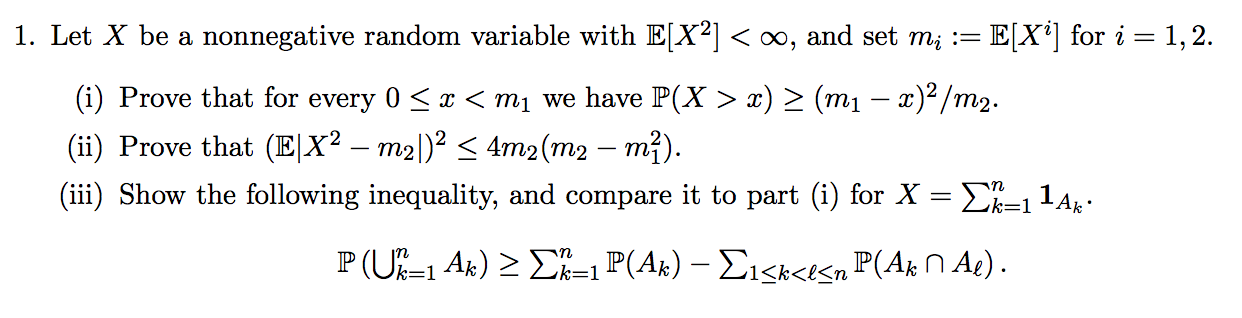
\includegraphics[width=0.7\textwidth]{problim-e2-p1.png}
\end{figure}
\end{question}
\begin{solution} \hfill \\
\textbf{(1)} Fix $\alpha \in [0,m_1)$. By Cauchy-Schwartz, 
\eQb
\mathbb{E}[1_{X > \alpha} X]^2 &\leq& \mathbb{E}[1_{\{X > \alpha\}}^2]
\mathbb{E}[ X^2] = \mathbb{P}(X > \alpha) m_2.
\eQe
On the other hand,
\eQb
m_1 &=& \mathbb{E}[X1_{\{ X > \alpha\}}] + E[X1_{\{ X \leq \alpha \}}], 
\eQe
which implies
\eQb
(m_1 - \alpha)^ 2&\leq& \mathbb{E}[X1_{\{ X > \alpha\}}]^2.
\eQe
Combining the above inequality with the first one and re-arranging yield
\eQb
\dfrac{(m_1 - \alpha)^2}{m_2} &\leq& \mathbb{P}(X > \alpha),
\eQe
as required. \hfill $\qed$

\bigskip
\textbf{(2)} By Cauchy-Schwartz, 
\eQb
\mathbb{E}[|(X+m_2^{\frac{1}{2}})(X-m_2^{\frac{1}{2}})|]  &\leq&
(\mathbb{E}[X^2 + 2{m_2}^{\frac{1}{2}}X + m_2] 
\mathbb{E}[X^2 - 2{m_2}^{\frac{1}{2}}X + m_2])^{\frac{1}{2}} \\
&=& (4{m_2}^2 - 4 m_2 {m_1}^2)^{\frac{1}{2}} = 2m_2^{\frac{1}{2}}
(m_2 - {m_1}^2)^{\frac{1}{2}}. \\
\eQe
Squaring both sides gives the desired inequality. \hfill $\qed$

\bigskip


\textbf{(3)} We show the inequality via induction. For $n = 2$, 
\eQb
\mathbb{P}(A_1 \cup A_2) &=& \mathbb{P}({A_1}^c \cap A_2) + 
\mathbb{P}(A_1 \cap {A_2}^c) + \mathbb{P}(A_1 \cap A_2) \\
&=& \mathbb{P}({A_1}^c \cap A_2) + \mathbb{P}(A_1 \cap A_2)  
+ \mathbb{P}(A_1 \cap {A_2}^c) + \mathbb{P}(A_1 \cap A_2) 
- \mathbb{P}(A_1 \cap A_2) \\
&=& \mathbb{P}(A_1) + \mathbb{P}(A_2) - \mathbb{P}(A_1 \cap A_2).
\eQe
Now, suppose the statement is true for some $n > 2$. Then,
using the $n=2$ case, the inductive hypothesis and subadditivity gives
\eQb
\mathbb{P}(\bigcup_{k=1}^{n+1} A_k) &=& \mathbb{P}(\bigcup_{k=1}^{n} A_k \bigcup
A_{n+1}) \\
&=& \mathbb{P}(\bigcup_{k=1}^{n} A_k) + \mathbb{P}(A_{n+1}) - \mathbb{P}
(\bigcup_{k=1}^{n} A_k \bigcap A_{n+1}) \\
&\geq& \sum_{k=1}^{n} \mathbb{P}(A_k) - \sum_{1\leq k<l\leq n} 
\mathbb{P}(A_k \bigcap A_l) + \mathbb{P}(A_{k+1}) - \mathbb{P}(
\bigcup_{k=1}^{n} A_n \bigcap A_{n+1}) \\
&\geq& \sum_{k=1}^{n+1} \mathbb{P}(A_k) - \sum_{1\leq k<l\leq n} 
\mathbb{P}(A_k \bigcap A_l) - \sum_{k=1}^{n} \mathbb{P}(
A_k \bigcap A_{n+1}) \\
&=& \sum_{k=1}^{n+1} \mathbb{P}(A_k) - \sum_{1 \leq k< l \leq n} 
\mathbb{P}(A_k \bigcap A_l). 
\eQe
Therefore, the induction is complete and the inequality is true.
Now, if $X = \sum_{k=1}^{n} 1_{A_k}$, then
\eQb
m_1 &=& E[X] = \sum_{k=1}^{n} \mathbb{P}(A_n) \\
m_2 &=& E[X^2] = \mathbb{E}[\sum_{1\leq k<l\leq n}1_{A_k}] = \sum_{1 \leq k < l \leq n}
\mathbb{P}(A_k \cap A_l) 
\eQe
and
\eQb
\mathbb{P}(X > \alpha) &=& \mathbb{P}(\bigcup_{k=1}^{n} A_k),
\eQe
for any $\alpha \in (0,1]$. Hence, to compare, if $X = \sum_{k=1}^{n} 1_{A_k}$,
we can re-write $(iii)$ as
\eQb
P(X > \alpha) &\geq& m_1 - m_2,
\eQe
for any $\alpha \in (0,1]$. \hfill $\qed$

\end{solution}

\newpage

\begin{question}[2]
\hfill
\begin{figure}[h!]
  \centering
    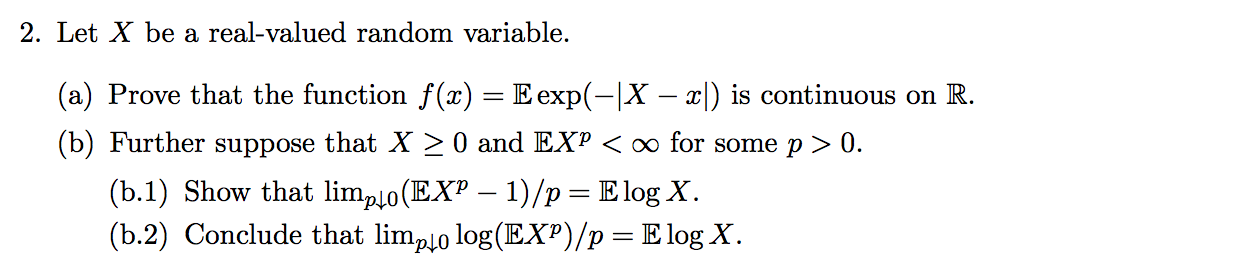
\includegraphics[width=0.7\textwidth]{problim-e2-p2.png}
\end{figure}
\end{question}
\begin{solution} \hfill \\
\textbf{(a)}
We first note that, for any $x \in \mathbb{R}$,
$\exp(-|X - x|)$ is uniformly bounded by $1$, and we have a finite measure,
so the expectation is well-defined and $f$ is well-defined everywhere.
Set $\mu = L(X)$. Then, by a change of variable,
\eQb
f(x) &=& \mathbb{E}[\exp(-|X-x|) = \int_{-\infty}^{\infty} \exp(-|t-x|)\mu(dt) 
\eQe
so, for $x,h \in \mathbb{R}$,
\eQb
|f(x+h) - f(x)| &=& |\int e^{-|t - x - h|} - e^{-|t - x|} \mu(dt) | \\  
&\leq& \int |e^{-|t-x-h|} - e^{-|t-x|}| \mu(dt) \>\>\> (*).
\eQe
Observe that
\eQb
|e^{-|t-x-h|} - e^{-|t-x|}| \leq 2 
\eQe
for any $t,x,h \in \mathbb{R}$
and
\eQb
| e^{-|t-x-h|} - e^{-|t-x|}| \to 0 \>\> \text{as} \>\> h \to 0 
\eQe
for any $t,x \in \mathbb{R}$.
Therefore, by BCT and (*), it follows that
\eQb
|f(x+h) - f(x)| \to 0 \>\> \text{as} \>\> h \to 0,
\eQe
which shows that $f$ is continuous as required. \hfill $\qed$

\bigskip

\textbf{(b.1)} With L'hopital's rule, we obtain that
\eQb
\lim_{p \downarrow 0} \dfrac{X^{p}(w) - 1}{p} &=& \lim_{p \downarrow 0}
X^p(w) \log(X(w)) = \log(X(w)),
\eQe
for all $w \in \Omega$. Hence,
\eQb
\{\dfrac{X^p - 1}{p}\}_{p \geq 0} \>\> \text{ converges almost surely to }
\log(X) \text{ on } \Omega
\eQe

 By DCT,
\eQb
\lim_{p \downarrow 0} \dfrac{(\mathbb{E}X^p -1)}{p} &=& \mathbb{E}\log(X),
\eQe 
as required. \hfill $\qed$

\bigskip

\textbf{(b.2)} 

\textbf{(Remark)} Although all limit theorems are stated so far
for a countable limit, they apply as well to a continuous limit. 
Suppose $\{X_t\}_{t \geq 0}$ is a family of $L^1$ dominated 
random variables such that $\lim_{t \downarrow 0}
X_t(w) \to X_0(w)$ for all $w \in \Omega$. Then, by DCT, for any $\{t_n\} \subset
(0,\infty)$ such that $t_n \downarrow 0$, 
we have $\lim_{n \to \infty} \mathbb{E}[X_{t_n}] = 
\mathbb{E}[X_0]$. Since this is true for any such sequence, it follows that
$\lim_{t \downarrow 0}\mathbb{E}[X_t] = \mathbb{E}[X_0]$ in a proper continuous limit
sense. We will freely use the limit theorem in the continuous setting without
doing the above pass everytime.


\end{solution}

\newpage

\begin{question}[3]
\hfill
\begin{figure}[h!]
  \centering
    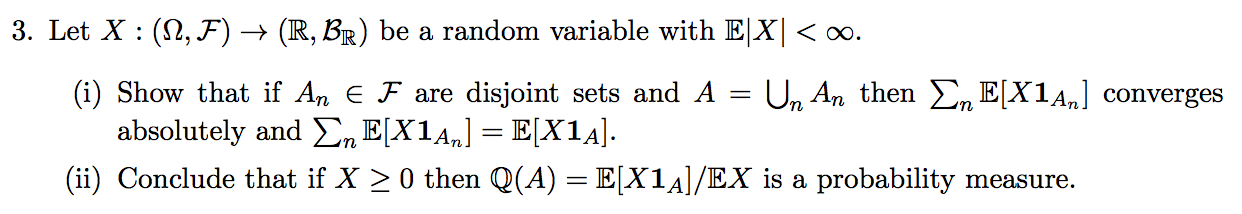
\includegraphics[width=0.7\textwidth]{problim-e2-p3.png}
\end{figure}
\end{question}
\begin{solution} \hfill \\
We first show the case for non-negative, simple functions. Let $X$ be simple, such that
\eQb
X &=& \sum_{k=1}^{l} a_k \mathbbm{1}_{E_k},
\eQe
where $a_k \in \mathbb{R}$ for $k = 1,...,l$ and $E_k \in \mathscr{F}$ 
with $\bigcupdot_{k=1}^{l} E_k = \Omega$. With linearity of expectation,
\eQb
\mathbb{E}[X\mathbbm{1}_{A}] &=& \mathbb{E}[\sum_{k=1}^{l} a_k \mathbbm{1}_{E_k}
\mathbbm{1}_{A}] 
= \sum_{k=1}^{l} a_k\mathbb{E}[\mathbbm{1}_{E_k} \mathbbm{1}_{A}] \\
&=& \sum_{k=1}^{l} a_k\mathbb{E}[\mathbbm{1}_{E_k \cap A}] 
= \sum_{k=1}^{l} a_k \mathbb{P}(E_k \cap A).
\eQe  
Similarly,
\eQb
\mathbb{E}[X\mathbbm{1}_{A_n}] &=& \sum_{k=1}^{l} a_k\mathbb{P}(E_k \cap A_n) 
\eQe
for each $n \geq 1$. Then, it follows that, for all $m \geq 1$,
\eQb
\sum_{n=1}^{m} |\mathbb{E}[X\mathbbm{1}_{A_n}]| &=& \sum_{n=1}^{m} \sum_{k=1}^{l} 
a_k \mathbb{P}(E_k \cap A_n) \\
&=& \sum_{k=1}^{l} a_k \mathbb{P}(E_k \cap \bigcup_{m\geq n} A_n), \\
\eQe
where the equality holds by disjointness of $\{A_n\}$. Since $\bigcup_n A_n = A$,
we can exploit continuity of probability and obtain 
\eQb
\sum_{n} |\mathbb{E}[X\mathbbm{1}_{A_n}]| &=& \lim_{m \to \infty} \sum_{k=1}^{l} a_k
\mathbb{P}(E_k \cap \bigcup_{m \geq n} A_n) \\
&=& \sum_{k=1}^{l} a_k \lim_{m \to \infty} \mathbb{P}(E_n \cap \bigcup_{m \geq n}
A_n) = \sum_{k=1}^{l} a_k \mathbb{P}(E_n \cap A) = \mathbb{E}[X\mathbbm{1}_A].
\eQe
Hence, we have shown that for $X$ non-negative and simple, $\sum_{n} 
\mathbb{E}[X\mathbbm{1}_{A_n}]$ converges absolutely to $\mathbb{E}[X\mathbbm{1}_{A}]$. 

\bigskip

We now extend the case to non-negative integrable functions. 
Let $X$ be a bounded, measurable, non-negative functions. Choose $\{ \phi_k\}$
simple functions such that $\phi_k \to X$. By the previous result, 
we observe
\eQb
\sum_{n} \mathbb{E}[\phi_k \mathbbm{1}_{A_n}] = \mathbb{E}[\phi_k \mathbbm{1}_{A}] 
\>\> (*)
\eQe
for any $k \geq 1$. Since $\phi_k \to X$ uniformly, by monotone convergence theorem,
\eQb
\mathbb{E}[\phi_k \mathbbm{1}_{A}] \to \mathbb{E}[\phi_k \mathbbm{1}_{A}]
\eQe
and
\eQb
\mathbb{E}[\phi_k \mathbbm{1}_{A_n}] \to \mathbb{E}[\phi_k \mathbbm{1}_{A_n}]
\eQe
which via implies
\eQb
\sum_{n} \mathbb{E}[\phi_k \mathbbm{1}_{A_n}] \to \sum_{n} 
\mathbb{E}[\phi_k \mathbbm{1}_{A_n}].
\eQe
Combining (*) with the above limit, we see that 
$\sum_{n} 
\mathbb{E}[X\mathbbm{1}_{A_n}]$ converges absolutely and 
$\sum_{n} 
\mathbb{E}[X\mathbbm{1}_{A_n}] = \mathbb{E}[\mathbbm{1}_{A}]$ as required.
By considering the positive part and negative part, we can extend the
result to any random variable as required. 

\textbf{(ii)} Firstly, observe that
\eQb
\mathbb{Q}(\Omega) &=& \dfrac{\mathbb{E}[\mathbbm{1}_{\Omega}]}{\mathbb{E}[X]} = 
\dfrac{\mathbb{E}[X]}{\mathbb{E}[X]} = 1.
\eQe
Hence, it now suffices to show that $\mathbb{Q}$ is countably additive, but from
the discussion in $(i)$, we see
\eQb
\mathbb{Q}(\bigcup_n A_n) &=& \dfrac{\mathbb{E}[X\mathbbm{1}_{\cup_n A_n}]}{
\mathbb{E}[X]}  
= \dfrac{\sum_{n} \mathbb{E}[X\mathbbm{1}_{A_n}]}
{\mathbb{E}[X]} = \sum_n \mathbb{Q}(A_n).
\eQe
for any $\{A_n\} \subset \mathscr{F}$ that are pairwise disjoint. So,
$\mathbb{Q}$ is a probability measure, if $X \geq 0$ and we are done
\hfill $\qed$
 
\end{solution}

\newpage

\begin{question}[4]
\hfill
\begin{figure}[h!]
  \centering
    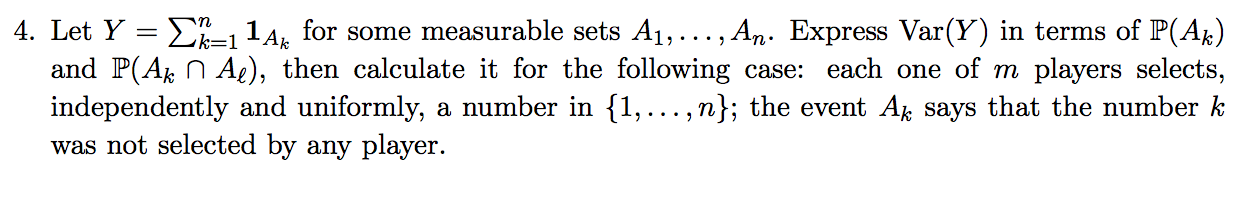
\includegraphics[width=0.7\textwidth]{problim-e2-p4.png}
\end{figure}
\end{question}
\begin{solution} \hfill \\
We compute
\eQb
\Var[Y] &=& \mathbb{E}[Y^2] - \mathbb{E}[Y]^2 \\
&=& \mathbb{E}[(\sum_{k=1}^{l} \mathbbm{1}_{A_k})^2] - \mathbb{E}[
\sum_{k=1}^{l} \mathbbm{1}_{A_k}]^2 \\
&=& \sum_{k=1}^{n} \sum_{l=1}^{n} \mathbb{E}[\mathbbm{1}_{A_k}\mathbbm{1}_{A_l}]
- \sum_{k=1}^{n} \sum_{l=1}^{n} \mathbb{E}[\mathbbm{1}_{A_k}] \mathbb{E}[
\mathbbm{1}_{A_l}] \\
&=& \sum_{k=1}^{n} \sum_{l=1}^{n} 
\mathbb{E}[\mathbbm{1}_{A_k \cap A_l}] - \mathbb{E}[\mathbbm{1}_{A_k}]
\mathbb{E}[\mathbbm{1}_{A_l}] \\
&=& \sum_{k=1}^{n} \sum_{l=1}^{n} \mathbb{P}(A_k \cap A_l) - \mathbb{P}(A_k)
\mathbb{P}(A_l).
\eQe
Now, observe that, for $k = 1,...,n$, 
\eQb
\mathbb{P}(A_k) &=& (\dfrac{n-1}{n})^m 
\eQe
and for $k,l = 1,...,n$,
\eQb
k = l &\implies& \mathbb{P}(A_k \cap A_l)  = (\dfrac{n-1}{n})^{m} \\
k \neq l &\implies& \mathbb{P}(A_k \cap A_l) = (\dfrac{n-2}{n})^{m}. \\ 
\eQe
So
\eQb
\Var[Y] &=& 
\sum_{1\leq k,l \leq n; k \neq l} (\dfrac{n-2}{n})^{m} - (\dfrac{n-1}{n})^{2m} 
+ \sum_{1 \leq k,l \leq n; k = l} (\dfrac{n-1}{n})^{m} - (\dfrac{n-1}{n})^{2m}  \\
&=& (n^2-n)(\dfrac{n-2}{n})^m +  n(\dfrac{n-1}{n})^m - n^2(\dfrac{n-1}{n})^{2m} 
\eQe
as required. \hfill $\qed$

\end{solution}

\end{document}
